% Owner: C | Page budget: 0.6 pages
% Limits: <=1.25 column, <=350 words, <=5 equations, <=1 figure + 1 table
\subsection{System Modeling}
\label{sec:modeling}

We model a box-in-box cell inspired by~\cite{kana2023boxinbox} in MuJoCo~\cite{todorov2012mujoco} ($1\text{ ms}$ step) with a 7-DoF torque-controlled Franka Panda~\cite{menagerie2022,frankadocs} (Fig.~\ref{fig:scene}). A rigid $30\times 30\times 60\text{ mm}$ peg ($0.2\text{ kg}$) is mounted on the flange behind a wrist force/torque (F/T) sensor and inserted into a fixed $40\text{ mm}$-deep square hole ($0.5\text{ mm}$ per-side clearance; $3\text{ mm}$, $45^\circ$ chamfer). All quantities are in SI units. The world frame $\{W\}$ is at the robot base ($z$ up) and the tool-centre-point (TCP) frame $\{T\}$ is at the peg end-face centre. For joint positions $q \in \mathbb{R}^7$, forward kinematics (FK) gives the TCP pose $x$ from the modified DH chain~\cite{frankadocs,menagerie2022}, and $J(q) \in \mathbb{R}^{6\times 7}$ maps $\dot{q}$ to the TCP twist $\dot{x}$ (linear $v$, angular $\omega$) in $\{W\}$:
\begin{equation}
\dot{x} = [v;\,\omega] = J(q)\dot{q}.
\label{eq:twist}
\end{equation}

\begin{figure}[t]
\centering
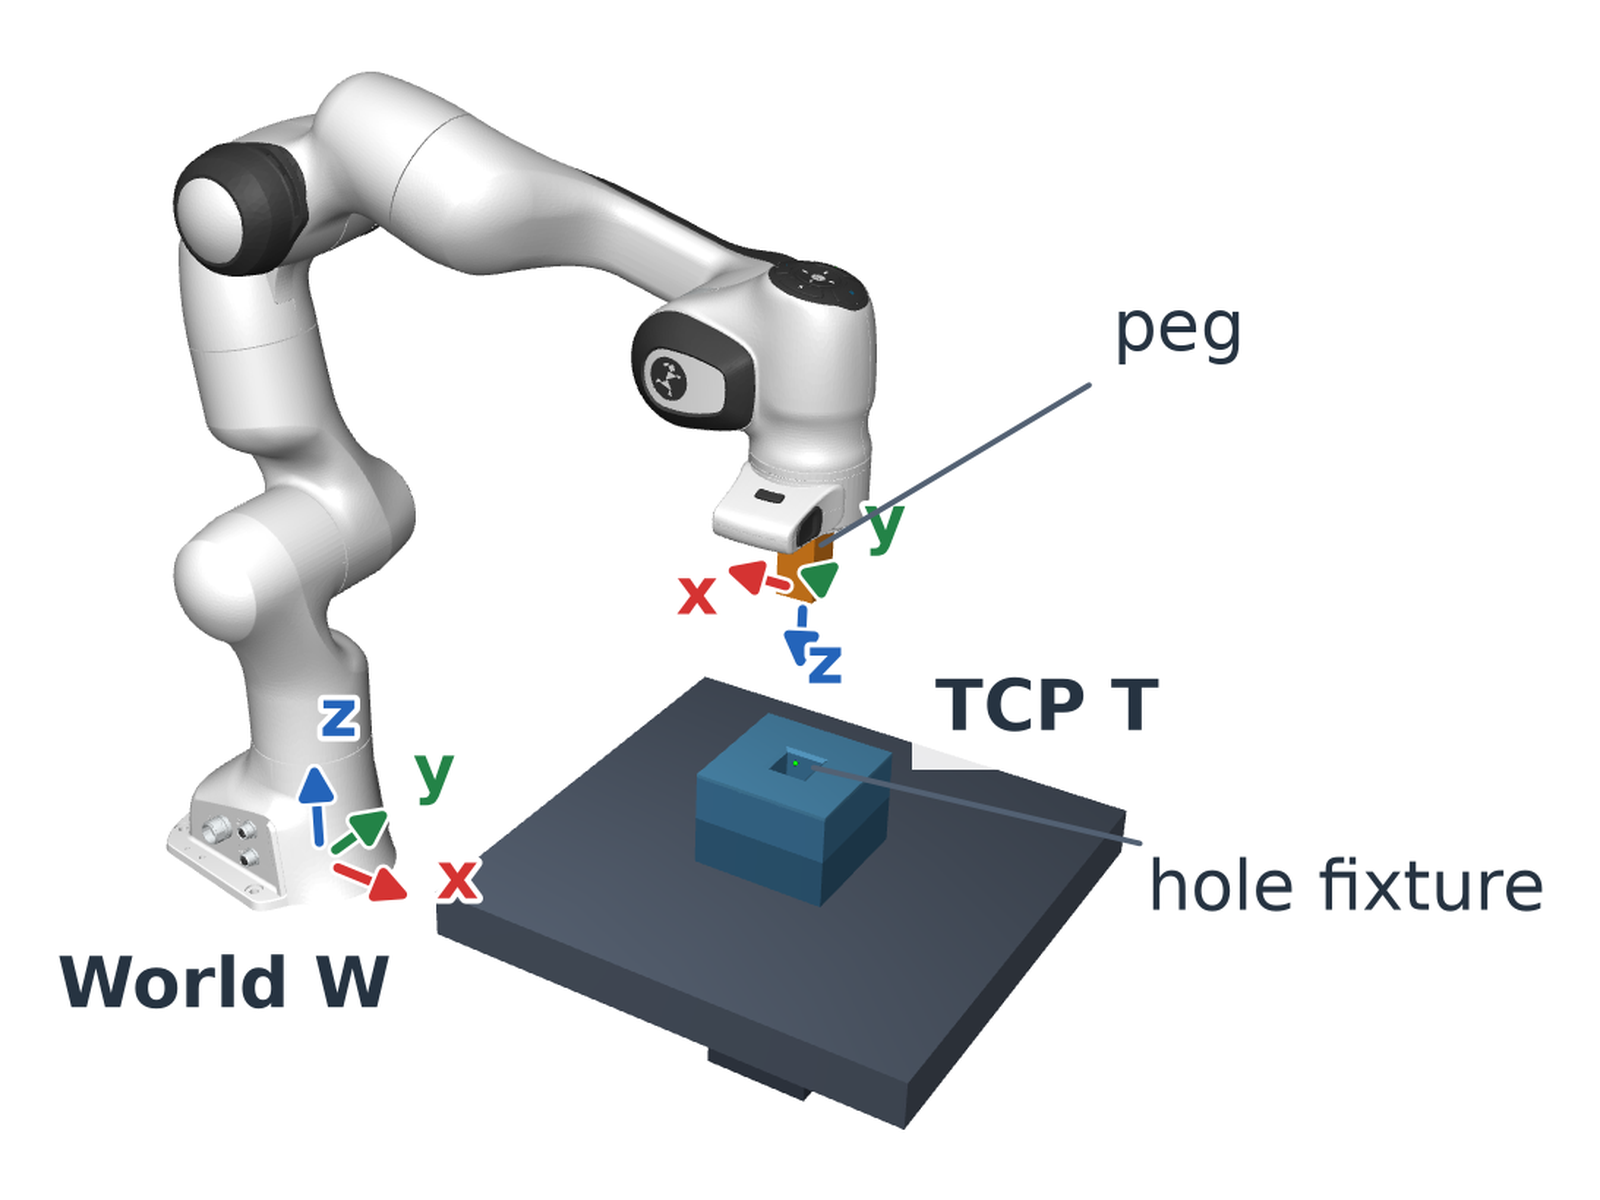
\includegraphics[width=0.6\columnwidth]{scene.png}
\caption{Simulated box-in-box setup with frames $\{W\}$ and $\{T\}$.}
\label{fig:scene}
\end{figure}

With rigid-body inertia $M_{rb}(q)$, armature $I_a = 0.1 I_7\text{ kg}\cdot\text{m}^2$, total inertia $\mathcal{M}(q) = M_{rb}(q) + I_a$, Coriolis term $h(q,\dot{q}) = C(q,\dot{q})\dot{q}$, gravity $g(q)$, viscous damping $D = 1.0 I_7\text{ N}\cdot\text{m}\cdot\text{s/rad}$, and external joint torque $\tau_{\text{ext}}$ ($= J^T F_{\text{ext}}$ for a wrench $F_{\text{ext}} \in \mathbb{R}^6$ applied by the environment at the TCP):
\begin{equation}
(M_{rb}(q) + I_a)\ddot{q} + C(q,\dot{q})\dot{q} + g(q) + D\dot{q} = \tau + \tau_{\text{ext}}.
\label{eq:joint_eom}
\end{equation}
The motor torque is the controller torque $\tau_{\text{cmd}}$ plus gravity compensation, saturated at the joint torque limits $\tau_{\max}$~\cite{frankadocs}: $\tau = \operatorname{clip}(\tau_{\text{cmd}} + g(q), -\tau_{\max}, +\tau_{\max})$. For task wrench $F \in \mathbb{R}^6$, null-space torque $\tau_0 \in \mathbb{R}^7$, $\ddot{x} = J\ddot{q} + \dot{J}\dot{q}$, and $\tau_{\text{cmd}} = J^T F + N_\tau \tau_0$, the operational-space dynamics~\cite{khatib1987unified} are
\begin{equation}
\Lambda\ddot{x} + \mu = F + F_{\text{ext}}, \qquad \mu = \mu_{rb} + \mu_D,
\label{eq:op_eom}
\end{equation}
with $A = J\mathcal{M}^{-1}J^T$, inertia $\Lambda$, dynamically consistent inverse $\bar{J}$ ($F_{\text{ext}} = \bar{J}^T \tau_{\text{ext}}$), and null-space torque projector $N_\tau$:
\begin{equation}
\Lambda = A^{-1}, \qquad \bar{J} = \mathcal{M}^{-1}J^T\Lambda, \qquad N_\tau = I_7 - J^T\bar{J}^T,
\label{eq:op_proj}
\end{equation}
where $\mu_{rb} = \Lambda(J\mathcal{M}^{-1}h - \dot{J}\dot{q})$, $\mu_D = \Lambda J\mathcal{M}^{-1}D\dot{q}$, and $A$ is regularized as $A + \lambda^2 I_6$ ($\lambda = 0.01$) for robustness near singularities.

The wrist F/T sensor gives $F_{\text{ext}}$ at $\{T\}$ in $\{W\}$ after tool gravity/inertia compensation. The simulator also provides the external joint torque $\tau_{\text{ext}}$, summed over all robot contacts through their contact Jacobians. Contacts use MuJoCo's soft-contact model (friction $0.3$) and a free $0.6\text{ kg}$ hand body whose contact is calibrated so that its impact peak force matches the ISO/TS~15066 hand model ($75\text{ N/mm}$) within $2\%$~\cite{iso15066} (Section~\ref{sec:safety}). Independent NumPy FK, $J$, $\mathcal{M}$, and $g$ match MuJoCo to machine precision (Table~\ref{tab:verification}). With $\lambda = 0$,~\eqref{eq:op_eom}--\eqref{eq:op_proj} reproduce simulated TCP accelerations over $1000$ well-conditioned random states within $2.92\times 10^{-12}\text{ m/s}^2\text{ (or rad/s}^2\text{)}$.

\begin{table}[t]
\centering
\caption{Model verification against MuJoCo and finite differences (max error over 1000 random states)}
\label{tab:verification}
% Generated: six data rows; scoped footnotesize for 252 pt IEEE columns.
{\footnotesize
\setlength{\tabcolsep}{2pt}
\begin{tabular}{@{}lll@{}}
\hline
Quantity & Reference & Max error \\
\hline
TCP pos. [m] & MuJoCo & $1.35\times10^{-15}$ \\
TCP rot. [rad] & MuJoCo & $1.03\times10^{-15}$ \\
$J$ [m/rad; 1] & MuJoCo / FD & $4.11\times10^{-15}$ / $3.40\times10^{-10}$ \\
$\mathcal{M}$ [1] & MuJoCo (rel.) & $3.04\times10^{-15}$ \\
$g$ [N m] & MuJoCo & $6.39\times10^{-14}$ \\
EOM [N m] & Fwd. / inv. & $2.63\times10^{-13}$ / $6.39\times10^{-14}$ \\
\hline
\end{tabular}
}

\end{table}
